\documentclass[conference]{IEEEtran}
\IEEEoverridecommandlockouts
% Based on the IEEE conference template (Overleaf: "IEEE Conference Template").
\usepackage{cite}
\usepackage{amsmath,amssymb,amsfonts}
\usepackage{algorithm}
\usepackage{algorithmic}
\usepackage{graphicx}
\usepackage{textcomp}
\usepackage{xcolor}
\usepackage{booktabs}
\usepackage{url}
\usepackage{tikz}
\usetikzlibrary{arrows.meta,positioning,fit,backgrounds}
\usepackage{pgfplots}
\pgfplotsset{compat=1.18}
\def\BibTeX{{\rm B\kern-.05em{\sc i\kern-.025em b}\kern-.08em
    T\kern-.1667em\lower.7ex\hbox{\sc e}\kern-.125emX}}

% Shared bar-chart style for the benchmark figures
\pgfplotsset{benchbar/.style={
    ybar, width=\columnwidth, height=3.9cm, bar width=10pt,
    symbolic x coords={XDP,TC,TC+FIB,Kernel,nft+IPVS,OVS,OVS-ct}, xtick=data,
    ymin=0, enlarge x limits=0.13, axis lines*=left,
    ymajorgrids, grid style={gray!25},
    nodes near coords, every node near coord/.append style={font=\scriptsize},
    tick label style={font=\scriptsize}, label style={font=\footnotesize}}}

\begin{document}

\title{In-Kernel Programmable Data Planes for SDN:\\
An eBPF/XDP Gateway with Stateful Firewalling and\\
L4 Load Balancing Compared with Open vSwitch}

% \author{\IEEEauthorblockN{Team 0}
% \IEEEauthorblockA{\textit{Department of Computer Science and Engineering} \\
% \textit{Indian Institute of Information Technology Dharwad}\\
% Dharwad, India \\
% patilyogeshgouda@gmail.com}}

\maketitle

\begin{abstract}
Software-Defined Networking (SDN) classically separates a controller from
switches that execute OpenFlow match--action tables. Cloud-native platforms
increasingly move this data plane into the operating-system kernel using the
extended Berkeley Packet Filter (eBPF) and the eXpress Data Path (XDP). This
paper designs, formally specifies, implements and evaluates such a data plane
for a gateway that combines a stateful firewall, a Layer-4 load balancer with
destination and source network address translation (DNAT/SNAT) and graceful
backend draining, and per-flow telemetry, in a single verified eBPF program
attachable at the XDP or the Traffic Control (TC) hook. A Python control plane
programs it at runtime through pinned BPF maps and a REST interface and
expires connection state like OpenFlow timeouts. The firewall judges
load-balanced traffic by the flow the client sees, which keeps VIP policies
consistent in both directions and prevents state that would expose backends
directly. The implementation passes 92 of 93 automated tests (one skipped by
a kernel test-harness limitation), including kernel-level packet tests that
check every rewritten checksum. We compare it with plain kernel routing, the
kernel's native stateful stack (nftables and IPVS), and Open vSwitch (OVS)
with stateless OpenFlow~1.3 rules and with connection tracking, over 10
interleaved, CPU-pinned rounds on emulated veth links. All stateful
configurations provide the required functions and spread load evenly. The
eBPF data plane reaches 9.4--9.9~Gbit/s of TCP throughput (28--31\% below
plain routing) and 506--559~kpps for 64-byte packets (22--29\% below plain
routing); at the TC hook this is statistically indistinguishable from
nftables with IPVS, while OVS with connection tracking is 10--19\% faster
owing to its flow cache. In-kernel microbenchmarks show a per-packet cost of
about 0.21--0.23~$\mu$s that does not grow from 0 to 10\,000 rules or from 0
to 60\,000 tracked connections, and a drop cost of 0.15~$\mu$s per packet.
We discuss why veth links mask XDP's driver-level advantage.
\end{abstract}

\begin{IEEEkeywords}
software-defined networking, eBPF, XDP, programmable data plane, load
balancing, stateful firewall, Open vSwitch, Mininet
\end{IEEEkeywords}

%=====================================================================
\section{Introduction}
%=====================================================================
SDN decouples the control plane, which decides how traffic should be handled,
from the data plane, which applies those decisions packet by packet
\cite{kreutz2015sdn,feamster2014road}. OpenFlow \cite{mckeown2008openflow}
standardized this split: a controller installs prioritized match--action
entries into the flow tables of switches such as Open vSwitch (OVS)
\cite{pfaff2015ovs}. The standard model is expressive for stateless
forwarding; stateful functions such as connection tracking and NAT are
provided through extensions, e.g., the \texttt{ct} and \texttt{nat} actions
of OVS backed by the kernel's connection tracker.

Cloud-native infrastructures have taken a different path. eBPF allows verified
programs to be loaded into a running Linux kernel and attached to networking
hooks, and XDP runs such programs in the network driver before the kernel
allocates its packet structure \cite{hoiland2018xdp,vieira2020ebpf}.
Production systems such as Cilium \cite{cilium} and Katran \cite{katran}, and
research frameworks such as Polycube \cite{miano2021polycube}, implement their
data planes this way. The controller--switch boundary of SDN thus becomes a
boundary between a user-space agent and kernel tables (BPF maps).

This paper does not claim the first eBPF implementation of a firewall or load
balancer---prior systems provide these functions (Section~\ref{sec:related}). Instead it
contributes a compact, \emph{formally specified} gateway pipeline and a
like-for-like comparison against the stateful alternatives available on the
same kernel. Our contributions are:
\begin{enumerate}
\item A single eBPF pipeline, attachable at the XDP or TC hook without
tail-call chaining, that parses Ethernet/VLAN/ARP/IPv4/TCP/UDP/ICMP, enforces
a stateful firewall over MAC and IPv4 rules, load-balances connections to a
virtual IP (VIP) with DNAT/SNAT and graceful backend draining, and maintains
per-flow telemetry (Section~\ref{sec:method}).
\item A formal model of rule matching, stateful admission over the
client-visible flow, backend selection, NAT state coupling, checksum
maintenance and connection expiry, which is exactly the logic the
implementation executes (Section~\ref{sec:model}).
\item A libbpf-based control plane with a CLI, a REST API and a connection
reaper analogous to OpenFlow idle and hard timeouts.
\item An evaluation against four baselines---plain kernel routing, the
kernel's native stateful subsystems (nftables with connection tracking and
IPVS), stateless OpenFlow~1.3 on OVS, and OVS with connection tracking---with
93 automated tests, repeated and interleaved benchmark runs with confidence
intervals, and in-kernel microbenchmarks of per-packet cost versus rule count
and connection-table occupancy (Sections~\ref{sec:setup}--\ref{sec:results}).
\end{enumerate}

%=====================================================================
\section{Related Work}
\label{sec:related}
%=====================================================================
\textit{SDN, OpenFlow and OVS.} Kreutz \textit{et al.}\ survey the SDN
architecture and its data-plane abstractions \cite{kreutz2015sdn}; Feamster
\textit{et al.}\ trace its history \cite{feamster2014road}. OpenFlow
\cite{mckeown2008openflow} defines the match--action switch model that OVS
\cite{pfaff2015ovs} implements with a user-space slow path and a kernel flow
cache; P4 \cite{bosshart2014p4} generalizes the data plane to
protocol-independent pipelines. Tu \textit{et al.}\ revisit the OVS data path
after ten years, including its eBPF and AF\_XDP variants \cite{tu2021ovs}, and
Oko extends OVS with stateful BPF filters placed in the OpenFlow pipeline
\cite{chaignon2018oko}.

\textit{eBPF and XDP network functions.} H{\o}iland-J{\o}rgensen
\textit{et al.}\ present the design of XDP \cite{hoiland2018xdp}, and Vieira
\textit{et al.}\ survey eBPF and XDP \cite{vieira2020ebpf}. Miano
\textit{et al.}\ report lessons from building network services with eBPF
\cite{miano2018creating}, build bpf-iptables, which reproduces iptables
semantics with an eBPF classifier \cite{miano2019bpfiptables}, and generalize
these ideas in Polycube, a framework of chained eBPF network functions
(firewall, NAT, load balancer, router) with a REST control plane
\cite{miano2021polycube}. Scholz \textit{et al.}\ quantify eBPF packet
filtering in Linux \cite{scholz2018filtering}. Cilium \cite{cilium} and Katran
\cite{katran} are production eBPF data planes for Kubernetes networking and L4
load balancing.

\textit{Kernel subsystems and classification.} Linux provides stateful
filtering through Netfilter/nftables with the \texttt{nf\_conntrack}
connection tracker \cite{nftables} and L4 load balancing through IPVS
\cite{zhang2000lvs}. Maglev \cite{eisenbud2016maglev} introduced consistent
hashing for software load balancers. Tuple Space Search
\cite{srinivasan1999tss} classifies packets by probing one exact-match hash
table per combination of wildcarded fields; our rule matcher is a fixed tuple
space with ten tuples (Section~\ref{sec:rules}).

\textit{Positioning.} Compared with Polycube and bpf-iptables, which favor
generality (arbitrary rule sets, chains of independent programs), our design
keeps all functions in one program and one set of maps, specifies their
interaction formally---in particular how firewall state, NAT state and
draining interact---and evaluates the result against the kernel's own
stateful subsystems and a stateful OVS configuration rather than only against
stateless forwarding. Mininet \cite{lantz2010mininet} is used for emulation;
because emulated hosts share one kernel, the eBPF program under test is the
real kernel program.

%=====================================================================
\section{Problem Scenario and System Model}
\label{sec:model}
%=====================================================================
\subsection{Scenario}
A gateway connects a client subnet $\mathcal{C}=\{c_1,\dots,c_4\}$
(10.0.1.0/24) and a backend subnet $\mathcal{S}=\{s_1,\dots,s_4\}$
(10.0.2.0/24). A service is published at the VIP $v=10.100.0.1$, port 80, and
must be served by the backends. The gateway must (i) forward all inter-host
traffic, (ii) enforce operator-defined allow/drop rules, (iii) distribute new
connections to the VIP across healthy backends while keeping each connection
on one backend, (iv) let operators drain a backend without breaking its
established connections, and (v) export packet and byte counters. Rules and
backend pools change at runtime without reloading the data plane.

\subsection{System Model}
Fig.~\ref{fig:arch} shows the architecture. Every host has a dedicated veth
link to the gateway (\textit{routed access}: /32 host routes and proxy ARP),
so every packet between any two hosts traverses the gateway data plane. The
data plane is a set of kernel functions sharing nine BPF maps; the control
plane reads and writes the same maps through the \texttt{bpf()} system call.
Table~\ref{tab:maps} maps the formal symbols used below to the maps.

\begin{figure}[t]
\centering
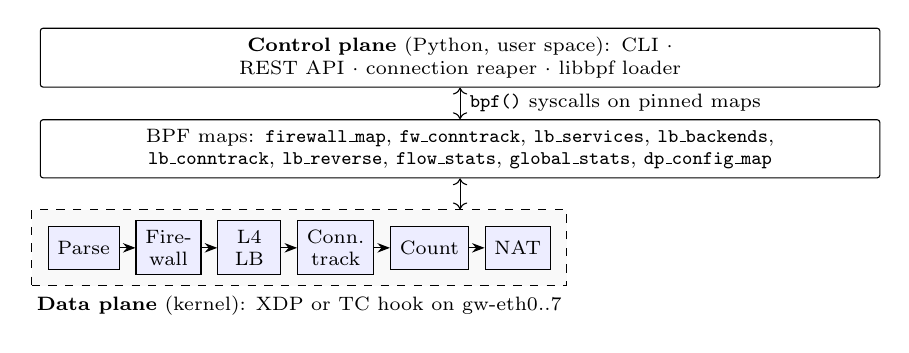
\begin{tikzpicture}[font=\scriptsize, node distance=2mm,
  box/.style={draw, rounded corners=1pt, align=center, minimum height=5mm, fill=white},
  stage/.style={draw, fill=blue!7, minimum height=5.5mm, minimum width=8mm, align=center},
  arr/.style={-{Stealth[length=1.6mm]}}]
\node[box, text width=0.86\columnwidth] (cp) {\textbf{Control plane} (Python, user space):
  CLI $\cdot$ REST API $\cdot$ connection reaper $\cdot$ libbpf loader};
\node[box, below=4mm of cp, text width=0.86\columnwidth] (maps)
  {BPF maps: \texttt{firewall\_map}, \texttt{fw\_conntrack}, \texttt{lb\_services},
   \texttt{lb\_backends},\\ \texttt{lb\_conntrack}, \texttt{lb\_reverse},
   \texttt{flow\_stats}, \texttt{global\_stats}, \texttt{dp\_config\_map}};
\node[stage, below=6mm of maps.south west, anchor=north west, xshift=1mm] (p) {Parse};
\node[stage, right=of p] (f) {Fire-\\wall};
\node[stage, right=of f] (l) {L4\\LB};
\node[stage, right=of l] (c) {Conn.\\track};
\node[stage, right=of c] (t) {Count};
\node[stage, right=of t] (n) {NAT};
\draw[arr] (p) -- (f); \draw[arr] (f) -- (l); \draw[arr] (l) -- (c);
\draw[arr] (c) -- (t); \draw[arr] (t) -- (n);
\begin{scope}[on background layer]
\node[draw, dashed, fill=gray!5, inner sep=2mm, fit=(p)(n),
  label={[font=\scriptsize]below:\textbf{Data plane} (kernel): XDP or TC hook on gw-eth0..7}] (dp) {};
\end{scope}
\draw[arr, <->] (cp) -- node[right] {\texttt{bpf()} syscalls on pinned maps} (maps);
\draw[arr, <->] (maps.south) -- (maps.south |- dp.north);
\end{tikzpicture}
\caption{Architecture: a user-space control plane programs a kernel data
plane through shared BPF maps.}
\label{fig:arch}
\end{figure}

\begin{table}[t]
\caption{Formal symbols and their BPF maps}
\label{tab:maps}
\centering\scriptsize
\setlength{\tabcolsep}{3pt}
\begin{tabular}{@{}lll@{}}
\toprule
Symbol & Map (type) & Content \\
\midrule
$\mathcal{R}$ & \texttt{firewall\_map} (hash) & rules: (pattern, fields) $\mapsto$ action, hits \\
$\mathcal{T}_{fw}$ & \texttt{fw\_conntrack} (LRU hash) & tracked flows, timestamps, TCP flags \\
$\sigma$ & \texttt{lb\_services} (hash) & $(v,p_v,\pi) \mapsto$ service id, pool size \\
$B_\sigma$, $\alpha$ & \texttt{lb\_backends} (array) & backend address, port, activity flag \\
$\mathcal{L}$ & \texttt{lb\_conntrack} (LRU hash) & client flow $\mapsto$ chosen backend \\
$\mathcal{T}_{rev}$ & \texttt{lb\_reverse} (LRU hash) & reply key $\mapsto (v,p_v)$ \\
-- & \texttt{flow\_stats} (per-CPU LRU hash) & per-flow packets, bytes \\
-- & \texttt{global\_stats} (per-CPU array) & 13 pipeline counters \\
$\delta$, $\gamma$ & \texttt{dp\_config\_map} (array) & default action, tracking on/off \\
\bottomrule
\end{tabular}
\end{table}

\subsection{Flows and Rules}
\label{sec:rules}
An IPv4 packet $x$ carries the flow key
\begin{equation}
f(x) = (s, d, p_s, p_d, \pi),
\end{equation}
with addresses $s,d$, ports $p_s,p_d$ and protocol $\pi$. Let $\rho(x)=1$ iff
$x$ is TCP or UDP and not a non-first IPv4 fragment, i.e., iff it carries
ports; otherwise $p_s=p_d=0$, so ICMP is matched on $(s,d,\pi)$ only. The
reverse key is $\bar f = (d, s, p_d, p_s, \pi)$.

Rules follow ten \emph{patterns}. Pattern $i$ selects a subset of fields, and a
rule is stored under the key $(i, m_i(\cdot))$; the pattern id is part of the
key, so an unselected field is a true wildcard and a packet whose port or
protocol happens to be zero can never match a wildcarded rule by accident. In
lookup order:
\begin{equation}
\begin{aligned}
&m_1{:}\,(\mathrm{mac}_s,\mathrm{mac}_d),\;\; m_2{:}\,(\mathrm{mac}_s),\;\;
 m_3{:}\,(s,d,p_s,p_d,\pi)^{\rho},\\
&m_4{:}\,(s,d,p_d,\pi)^{\rho},\;\; m_5{:}\,(s,d,p_s,\pi)^{\rho},\;\;
 m_6{:}\,(s,d,\pi),\\
&m_7{:}\,(s,d),\;\; m_8{:}\,(d,p_d,\pi)^{\rho},\;\; m_9{:}\,(s),\;\;
 m_{10}{:}\,(d),
\end{aligned}
\label{eq:patterns}
\end{equation}
where $^{\rho}$ marks patterns tried only if $\rho(x)=1$. The L2 patterns
$m_1,m_2$ apply to every Ethernet frame (including IPv6 and other non-IP
traffic); $m_3$--$m_{10}$ apply to IPv4 only. Pattern $m_8$ expresses a
service rule such as ``any client may reach $v$:80/TCP''. The order is a
total priority order, like OpenFlow priorities: where two patterns are
incomparable in specificity ($m_4$/$m_5$, $m_9$/$m_{10}$) the earlier one
wins, and an operator who needs the opposite outcome adds a more specific
rule. The matched action for a key $k$ is
\begin{equation}
A(k) = a\big(i^*, m_{i^*}(k)\big),\quad
i^* = \min\{\, i : (i, m_i(k)) \in \mathcal{R} \,\},
\label{eq:match}
\end{equation}
and $A(k)=\textsc{none}$ if no pattern matches. $A_2(x)$ denotes the result
over $m_1,m_2$ only.

\subsection{Client-Visible Flow and Stateful Admission}
The firewall judges load-balanced traffic by the flow the client sees. For a
reply from a backend, $f(x)$ carries the backend's real address; we define
the client-visible key
\begin{equation}
\kappa(x) = \begin{cases}
(v, d, p_v, p_d, \pi) & \text{if } \mathcal{T}_{rev}[f(x)] = (v,p_v),\\
f(x) & \text{if } f(x) \notin \mathcal{T}_{rev}.
\end{cases}
\label{eq:kappa}
\end{equation}
Forward packets to the VIP already carry $(c, v, p_c, p_v, \pi)$. Hence rules
written against the VIP apply in both directions, a rule between a client and
a specific backend does not affect traffic through the VIP, and no firewall
state is ever created for a backend's real address (which would otherwise
open a path from the client to the backend that bypasses the VIP policy).

Let $\gamma\in\{0,1\}$ indicate whether connection tracking is enabled and
$\delta$ the default action. A flow is \emph{established} iff $E(k)=1$, where
$E(k) = \mathbb{1}\big[\gamma = 1 \land (k \in \mathcal{T}_{fw} \lor \bar k \in
\mathcal{T}_{fw})\big]$. Non-IPv4 frames (ARP, IPv6, \dots) are admitted iff
$A_2(x) \ne \textsc{drop}$, independently of $\delta$, so IP policy cannot
break address resolution. An IPv4 packet with $k=\kappa(x)$ is admitted iff
$A_2(x) \ne \textsc{drop}$ and
\begin{equation}
\mathrm{adm}(x) =
\begin{cases}
0 & A(k) = \textsc{drop},\\
1 & A(k) = \textsc{allow},\\
1 & A(k) = \textsc{none} \land \delta=\textsc{allow},\\
E(k) & A(k) = \textsc{none} \land \delta = \textsc{drop}.
\end{cases}
\label{eq:adm}
\end{equation}
An explicit \textsc{drop} rule therefore takes effect immediately, even on
established connections. After an admitted packet has also passed the load
balancer, and if $\gamma=1$, the tracker refreshes the entry of $k$ if
$k\in\mathcal{T}_{fw}$; otherwise it refreshes the entry of $\bar k$ and marks
it as having seen a reply if $\bar k\in\mathcal{T}_{fw}$; otherwise it
inserts $k$. Each connection thus occupies one entry, with one pair of
timestamps and the TCP flags of both directions.

\subsection{Load-Balancing Model}
A service $\sigma=(v,p_v,\pi)$ owns an ordered backend pool
$B_\sigma=(b_0,\dots,b_{n-1})$, $n \le 16$, where each backend
$b_j=(a_j, p_j)$ has an address and a port, and a drain flag
$\alpha_j\in\{0,1\}$. For a new connection $f$, the gateway computes a hash
$h(f)$ (Bob Jenkins' \textit{jhash} final mix over $s$, $d$ and the
port/protocol word), lets $r = h(f) \bmod n$ and, provided
$\sum_{j=0}^{n-1}\alpha_j > 0$, selects
\begin{equation}
\begin{aligned}
j^*(f) &= (r + k^*) \bmod n, \\
k^* &= \min\{\, k \in \{0,\dots,n-1\} : \alpha_{(r + k) \bmod n} = 1 \,\};
\end{aligned}
\label{eq:select}
\end{equation}
if $\sum_j\alpha_j = 0$, the packet is dropped. The choice is stored as
$\mathcal{L}[f]=(b_{j^*}, j^*)$.

\textit{Stickiness and graceful draining.} For a later packet of $f$ with
$\mathcal{L}[f]=(b,j)$, the stored backend is reused as long as slot $j$ still
holds $b$ (same address and port), \emph{regardless of} $\alpha_j$: draining
($\alpha_j \gets 0$) excludes $b_j$ from Eq.~(\ref{eq:select}) for new
connections only, while established connections continue until they close or
expire. Only if the backend was removed or replaced is $f$ re-selected; the
reverse entry of the old backend is deleted first.

If $h$ is uniform, the number of connections $N_j$ received by each of $n$
active backends out of $N$ satisfies $\mathbb{E}[N_j]=N/n$, which we test with
Pearson's statistic
\begin{equation}
\chi^2 = \sum_{j=0}^{n-1} \frac{(N_j - N/n)^2}{N/n}, \qquad
\text{d.o.f.} = n-1.
\label{eq:chi2}
\end{equation}

\subsection{Address Translation and State Coupling}
\label{sec:coupling}
For a client flow $f=(c,v,p_c,p_v,\pi)$ assigned to backend $b=(a_b,p_b)$, the
forward packet is rewritten by DNAT, $T_D(f)=(c,a_b,p_c,p_b,\pi)$, and the
reverse-NAT table records the key of the expected reply,
$\mathcal{T}_{rev}[r(f)] = (v,p_v)$ with $r(f)=(a_b,c,p_b,p_c,\pi)$. A reply
matching this key is rewritten by SNAT to $(v,c,p_v,p_c,\pi)$, so the client
only ever observes the VIP. Because $r(f)$ does not contain $(v,p_v)$, the
mapping is injective only if backend endpoints are disjoint across services;
the control plane enforces this invariant when a service is created.

$\mathcal{L}[f]$ and $\mathcal{T}_{rev}[r(f)]$ live in separate LRU maps, so
both directions maintain both entries: a forward packet refreshes
$\mathcal{L}[f]$ and refreshes---or, if the LRU evicted it,
re-creates---$\mathcal{T}_{rev}[r(f)]$; a reply refreshes
$\mathcal{T}_{rev}[r(f)]$ and $\mathcal{L}[f]$ and records a server FIN or RST
in $\mathcal{L}[f]$. A server-to-client download therefore keeps the
connection alive, and a server-initiated close shortens its timeout.

\subsection{Incremental Checksum Maintenance}
Rewriting addresses and ports invalidates the IPv4 header checksum and the
TCP/UDP checksum, whose pseudo-header covers both addresses. Recomputing them
costs $O(L)$ for a packet of length $L$. We use the incremental update of
RFC~1624 \cite{rfc1624}: if 16-bit words $m_i$ change to $m_i'$,
\begin{equation}
HC' = {\sim}\Big({\sim}HC \oplus \textstyle\bigoplus_i {\sim}m_i
\oplus \bigoplus_i m_i'\Big),
\label{eq:csum}
\end{equation}
where $\oplus$ is 16-bit ones'-complement addition (end-around carry)
\cite{rfc1071} and ${\sim}$ is bitwise complement; the cost is $O(1)$. For
the IPv4 header the changed words are the two halves of one address; for the
L4 checksum they are the address (via the pseudo-header) and the port. The
implementation accumulates the sum in 32 bits with \texttt{bpf\_csum\_diff},
folds the carries into 16 bits and complements the result. The only special
case is UDP (RFC~768 \cite{rfc768}): a received checksum of zero (``not
computed'') is left unchanged, and a computed UDP checksum of
\texttt{0x0000} is transmitted as \texttt{0xFFFF}; IPv4 header and TCP
checksums are written as computed.

\subsection{Connection Expiry}
Each tracked entry $e$ stores its creation time $\tau_c(e)$, last-seen time
$\tau_\ell(e)$ (both from \texttt{bpf\_ktime\_get\_ns}) and the TCP flags seen
in either direction. With the idle limit $\Theta(e) = T_{fin}$ if FIN or RST
has been seen and $T_{idle}$ otherwise, the entry is removed at reaper time
$t$ iff
\begin{equation}
t - \tau_\ell(e) > \Theta(e)
\;\lor\; \big(T_{hard} > 0 \,\land\, t - \tau_c(e) > T_{hard}\big),
\label{eq:expiry}
\end{equation}
which mirrors OpenFlow's \texttt{idle\_timeout} and \texttt{hard\_timeout}.
Removing $\mathcal{L}[f]$ also removes $\mathcal{T}_{rev}[r(f)]$.

%=====================================================================
\section{Proposed Methodology}
\label{sec:method}
%=====================================================================
\subsection{Data-Plane Pipeline}
Algorithm~\ref{alg:pipeline} gives the per-packet processing. It is written
once and called by both entry points (\texttt{xdp\_dataplane} and
\texttt{tc\_dataplane}); only the final rewrite differs between hooks. Every
header access is preceded by an explicit bounds check against the end of the
packet, which lets the in-kernel verifier prove memory safety. Malformed
headers (truncated, $\mathrm{IHL}<5$, inconsistent total length) are dropped.
The parser accepts one 802.1Q/802.1ad VLAN tag. Updates of the 13 global
counters are omitted from the algorithm for brevity.

\textit{Fragments.} The gateway does not reassemble IPv4 fragments. A
non-first fragment has $\rho(x)=0$: it skips the port patterns, is matched on
$(s,d,\pi)$, is tracked under the key $(s,d,0,0,\pi)$, and is neither
load-balanced nor NAT-rewritten.

\begin{algorithm}[t]
\caption{Per-packet data-plane pipeline}
\label{alg:pipeline}
\begin{algorithmic}[1]
\REQUIRE packet $x$, configuration $(\delta,\gamma,\text{flags})$
\STATE $(f,\text{ok}) \gets \textsc{Parse}(x)$ \COMMENT{bounds-checked}
\IF{\textbf{not} ok}
  \RETURN \textsc{Drop} \COMMENT{malformed}
\ENDIF
\IF{$A_2(x) = \textsc{drop}$}
  \RETURN \textsc{Drop} \COMMENT{L2 rules, every frame}
\ENDIF
\IF{$x$ is not IPv4}
  \RETURN \textsc{Pass} \COMMENT{ARP, IPv6, \dots}
\ENDIF
\STATE $k \gets \kappa(x)$ \COMMENT{Eq.~(\ref{eq:kappa})}
\IF{$\mathrm{adm}(x)=0$ (Eq.~(\ref{eq:adm}))}
  \RETURN \textsc{Drop}
\ENDIF
\STATE $\nu \gets \textsc{LoadBalance}(f)$ \COMMENT{Algorithm~\ref{alg:lb}}
\IF{$\nu = \textsc{NoBackend}$}
  \RETURN \textsc{Drop}
\ENDIF
\IF{$\gamma=1$}
  \STATE refresh $k$ or $\bar k$ in $\mathcal{T}_{fw}$, or insert $k$
\ENDIF
\STATE add $x$ to the per-flow counters of $f$
\IF{$\nu$ is a DNAT or SNAT rewrite}
  \STATE rewrite address and port; update checksums (Eq.~(\ref{eq:csum}))
\ENDIF
\IF{FIB forwarding enabled \textbf{and} route lookup succeeds}
  \STATE decrement TTL, rewrite MACs, \RETURN \textsc{Redirect}(egress)
\ENDIF
\RETURN \textsc{Pass}
\end{algorithmic}
\end{algorithm}

\subsection{Load Balancing and NAT}
Algorithm~\ref{alg:lb} implements Eq.~(\ref{eq:select}), graceful draining and
the state coupling of Section~\ref{sec:coupling}. The probing loop is bounded by the
constant 16, which lets the verifier prove termination. The connection tables
are LRU hash maps with 65\,536 entries each, so they cannot fill up and stop
admitting new connections.

\begin{algorithm}[t]
\caption{\textsc{LoadBalance}$(f)$, $f=(s,d,p_s,p_d,\pi)$}
\label{alg:lb}
\begin{algorithmic}[1]
\IF{$f \in \mathcal{T}_{rev}$}
  \STATE $(v,p_v) \gets \mathcal{T}_{rev}[f]$;
         $g \gets (d, v, p_d, p_v, \pi)$ \COMMENT{client flow}
  \STATE refresh $\mathcal{T}_{rev}[f]$ and $\mathcal{L}[g]$ (time, TCP flags)
  \RETURN SNAT $(s,p_s) \to (v,p_v)$
\ENDIF
\IF{$\rho(x)=0$ \textbf{or} $(d,p_d,\pi)$ is not a service}
  \RETURN \textsc{None}
\ENDIF
\STATE let $B_\sigma=(b_0,\dots,b_{n-1})$ be the pool of service $(d,p_d,\pi)$
\IF{$\mathcal{L}[f]=(b,j)$ exists \textbf{and} $b_j = b$}
  \STATE refresh $\mathcal{L}[f]$; refresh or re-create $\mathcal{T}_{rev}[r(f)]$
\ELSE
  \IF{$\mathcal{L}[f]$ exists}
    \STATE delete the stale reverse entry of its old backend
  \ENDIF
  \STATE $b \gets \bot$
  \FOR{$k=0$ \TO $\min(n,16)-1$}
    \STATE $j \gets (h(f) \bmod n + k) \bmod n$
    \IF{$\alpha_j = 1$}
      \STATE $(b, j^*) \gets (b_j, j)$; \textbf{break}
    \ENDIF
  \ENDFOR
  \IF{$b = \bot$}
    \RETURN \textsc{NoBackend}
  \ENDIF
  \STATE $\mathcal{L}[f] \gets (b,j^*)$;
         $\mathcal{T}_{rev}[r(f)] \gets (d,p_d)$
\ENDIF
\STATE $(a_b, p_b) \gets b$
\RETURN DNAT $(d,p_d) \to (a_b,p_b)$
\end{algorithmic}
\end{algorithm}

\subsection{Hook-Specific Rewriting}
At the XDP hook the program edits the packet in place. It updates the IPv4
header checksum with one \texttt{bpf\_csum\_diff} call over the 4-byte old
and new address, and the TCP/UDP checksum with a second call over 8~bytes:
the address (pseudo-header) followed by the 32-bit port word, since TCP and
UDP headers both begin with $(p_s,p_d)$. At the TC hook it uses
\texttt{bpf\_l3\_csum\_replace} and \texttt{bpf\_l4\_csum\_replace} with the
pseudo-header flag; these helpers also handle packets whose transport
checksum has not yet been finalized because of checksum offload. Optional
FIB forwarding queries the kernel routing table with \texttt{bpf\_fib\_lookup},
decrements the TTL with an incremental header-checksum update, rewrites both
MAC addresses and redirects the packet to the egress interface, bypassing the
IP stack; packets with $\mathrm{TTL}\le1$ or without a resolved neighbor are
passed to the stack.

\subsection{Telemetry}
Per-flow counters live in a per-CPU LRU hash map keyed by the exact flow key
(16\,384 entries), so flows never share an entry; when the map is full, the
least recently used flow is evicted. Only admitted packets are counted, so a
flood of dropped packets cannot evict legitimate flows; drops are counted in
the global counters, which use a per-CPU array. Per-CPU storage avoids atomic
operations; the control plane sums the per-CPU values when reading.

\subsection{Control Plane}
The control plane is written in Python and calls \texttt{libbpf} directly
through \texttt{ctypes}. It compiles the program with
\texttt{clang -O2 -target bpf}, loads it, pins all maps under
\texttt{/sys/fs/bpf} so that every CLI call and the daemon share one state,
and attaches the program to each gateway interface. Map layouts are mirrored as
\texttt{ctypes} structures whose sizes are asserted against the C definitions
at import time. Rules are validated against the ten patterns of
Eq.~(\ref{eq:patterns}); a rule of any other shape is rejected rather than
silently widened. Adding a \textsc{drop} rule flushes matching entries of
$\mathcal{T}_{fw}$ and $\mathcal{L}$, and the entries of $\mathcal{T}_{rev}$
whose client-visible flow matches, so established connections cannot bypass
the new policy. A daemon serves a JSON REST API and runs a reaper thread that
applies Eq.~(\ref{eq:expiry}).

\textit{Reaper consistency.} User space cannot atomically test and delete a
map entry, so the reaper re-reads each candidate immediately before deleting
it and skips it if a packet refreshed it in the meantime. A residual window of
microseconds remains; since an entry is only deleted after at least
$\Theta(e)$ seconds without traffic, a packet must arrive within that window
after a full idle period for the race to matter. If it does, the next forward
packet re-creates the state, and re-selection yields the same backend as long
as the pool is unchanged, because selection is a deterministic function of
$f$.

\subsection{Complexity}
\label{sec:complexity}
With hash maps, per-packet work is independent of the number of rules and
tracked connections: at most two L2 and eight IPv4 rule lookups, a constant
number of connection-table lookups, and at most $n \le 16$ backend lookups
for the first packet of a connection. Checksum maintenance is $O(1)$ by
Eq.~(\ref{eq:csum}). Section~\ref{sec:kernel-cost} measures this empirically.

%=====================================================================
\section{Baselines and Experimental Setup}
\label{sec:setup}
%=====================================================================
\subsection{Configurations}
We compare seven configurations of the gateway. Three use the proposed data
plane:
\begin{itemize}
\item \textbf{XDP}: the pipeline at the XDP hook (native veth XDP); packets are
passed to the kernel for routing.
\item \textbf{TC}: the same pipeline at the TC ingress hook.
\item \textbf{TC+FIB}: the TC hook with in-program forwarding via
\texttt{bpf\_fib\_lookup} and \texttt{bpf\_redirect}.
\end{itemize}
Four are baselines. Two are stateful and implement the same policy (stateful
firewall, VIP load balancing with DNAT/SNAT, graceful draining):
\begin{itemize}
\item \textbf{nft+IPVS}: the kernel's native subsystems---nftables with
connection tracking (drop rules ahead of an established-state accept, so a
drop rule wins over state, as in Eq.~(\ref{eq:adm})) and IPVS in NAT mode with
Maglev hashing on address and port \cite{zhang2000lvs,nftables}; draining sets
a backend's weight to 0.
\item \textbf{OVS-ct}: OVS with connection tracking: all IP traffic passes
\texttt{ct(nat)}; new connections to the VIP enter a \texttt{select} group
whose buckets perform \texttt{ct(commit,nat(dst=$b$))}; other new flows are
committed; established and related flows are routed. Draining removes the
backend's bucket with \texttt{mod-group}, and existing connections continue
through their conntrack NAT binding.
\end{itemize}
Two are stateless references:
\begin{itemize}
\item \textbf{Kernel}: Linux routing with the same addressing and no policy,
i.e., the cost of forwarding alone.
\item \textbf{OVS}: OpenFlow~1.3 rules only (firewall drops, a \texttt{select}
group for the VIP, stateless reverse NAT that rewrites every reply from a
backend's service port, routing). Without connection tracking it can drain
only by re-hashing existing connections.
\end{itemize}
Firewall drops are counted by the data plane in every configuration that has
a firewall: eBPF counters, the nftables rule counter, or the OpenFlow rule
counters (synchronized from the kernel datapath before reading).

\subsection{Testbed}
Experiments run in Mininet~2.3.1b4 \cite{lantz2010mininet} on a laptop with an
Intel Core i7-1355U (2 performance cores with 2 threads each, up to 5.0~GHz,
and 8 efficiency cores, up to 3.7~GHz) and 15~GiB of RAM, running Linux
7.2.15, with Clang~23.1.3 (\texttt{-O2}), libbpf~1.7.0, Open vSwitch~4.0.0,
nftables~1.1.7, ipvsadm~1.31 and iperf3~3.22; these versions are recorded
automatically with every run. The topology has one gateway, four clients and
four backends, each host on its own veth link to the gateway. Transmit
checksum offload is disabled on all veths, because a program at the XDP hook
otherwise sees transport checksums that hold only a partial pseudo-header
sum. This also disables TCP segmentation offload, so TCP is segmented into
1500-byte packets in software in every configuration; absolute TCP
throughput is therefore lower than on veth pairs with offloads enabled, but
the comparison is like for like. Each backend runs an HTTP server whose page
contains its own name, so every response identifies the serving backend. The
eBPF control-plane daemon runs with $T_{idle}=30$~s, $T_{fin}=5$~s and a
reaper period of 2~s.

\subsection{Correctness Methodology}
Functional correctness is evaluated at three levels: (i) 37 unit tests of the
control-plane logic against in-memory maps; (ii) 56 kernel tests (28 cases
$\times$ 2 hooks) that load the real programs and execute crafted packets with
\texttt{BPF\_PROG\_TEST\_RUN}, checking verdicts, rewritten headers and the
validity of every IPv4/TCP/UDP checksum, computed independently by the test,
and including one regression test per defect fixed in this revision (graceful
draining, stale reverse entries, reply-side refresh, re-creation of evicted
state, the client-visible firewall, service-port rules, L2 rules on non-IP
frames); and (iii) three Mininet scenarios for every configuration:
\textbf{T1} ping between all 56 ordered host pairs; \textbf{T2} a
bidirectional drop rule between $c_1$ and $s_3$, with $c_1 \to s_2$ required
to stay reachable, the data plane's drop counter required to increase, and
reachability restored after the rule is removed; \textbf{T3} 25 HTTP requests
from each client to the VIP (100 new TCP connections), requiring zero
failures and use of all backends, connection-tracking state, and---after
draining $s_1$---no new connections on $s_1$.

\subsection{Performance Methodology}
On the path $c_1 \to$ gateway $\to s_2$ we measure TCP throughput
(single-stream \texttt{iperf3}, 10~s); the received packet rate for 64-byte
frames (\texttt{iperf3} UDP with 22-byte payloads at unlimited rate, 10~s),
$\mathrm{pps}=(N_{sent}-N_{lost})/T$; round-trip time from 500 ICMP echoes at
2~ms intervals; and the new-connection rate through the VIP from 200
sequential HTTP requests. For configurations with a firewall we also flood a
blocked UDP port of $s_3$ from $c_1$ for 3~s and divide the increase of the
drop counter by the sender's own measured duration.

Every configuration was measured in 10 rounds; each round runs all seven
configurations once, each on a freshly built topology, so slow drift (e.g.,
thermal) affects all configurations alike. The CPU frequency governor is set
to \texttt{performance} for the whole run, and the traffic tools are pinned to
the first hardware threads of the two performance cores (client: CPU~0,
server: CPU~2). We report means with 95\% confidence intervals (Student's
$t$, 9 degrees of freedom) and compare configurations with Welch's
unequal-variance $t$-test.

Finally, an in-kernel microbenchmark times the loaded programs with
\texttt{BPF\_PROG\_TEST\_RUN}, which reports the kernel's own measurement of the
program's run time, independent of traffic generators: (a) the per-packet cost
of an admitted packet with 0 to 10\,000 installed rules, spread over all ten
patterns and none matching, so that every lookup level is probed (the worst
case); (b) the same cost with 0 to 60\,000 entries in each connection table;
and (c) the cost of each processing path (pass, firewall drop, DNAT, SNAT).
(a) and (b) use the kernel's repeat loop ($2\times10^5$ runs per sample, 15
samples). NAT rewrites the packet, so (c) runs each packet once per call
(20\,000 calls, 10 batch means) and therefore includes a constant timing
overhead, which is visible by comparing the pass path in (a) and (c).

%=====================================================================
\section{Results and Performance Analysis}
\label{sec:results}
%=====================================================================
\subsection{Functional Correctness}
All 37 unit tests pass. Of the 56 kernel tests, 55 pass and one is skipped:
for TC, the kernel's test harness refuses to construct a socket buffer from a
frame too short to hold an IPv4 header, so the truncated-frame case is
exercised only at the XDP hook (the TC program is still tested with an invalid
header length). In total, 92 of 93 automated tests pass and 1 is skipped.

Table~\ref{tab:correct} summarizes the Mininet scenarios. Both eBPF hooks and
both stateful baselines pass every check. Stateless OVS passes every check it
can express; it has no connection tracking. In T2, every data plane's drop
counter rose by exactly the three blocked echo requests.

\begin{table}[t]
\caption{Functional results of the Mininet scenarios}
\label{tab:correct}
\centering\scriptsize
\setlength{\tabcolsep}{2.4pt}
\begin{tabular}{@{}lccccc@{}}
\toprule
Check & XDP & TC & nft+IPVS & OVS & OVS-ct \\
\midrule
T1 all-pairs reachability (56 pairs) & pass & pass & pass & pass & pass \\
T2 $c_1 \leftrightarrow s_3$ blocked & pass & pass & pass & pass & pass \\
T2 $c_1 \to s_2$ still reachable & pass & pass & pass & pass & pass \\
T2 drops counted by the data plane & pass & pass & pass & pass & pass \\
T2 reachability restored & pass & pass & pass & pass & pass \\
T3 100/100 requests answered & pass & pass & pass & pass & pass \\
T3 all four backends used & pass & pass & pass & pass & pass \\
T3 connection tracking populated & pass & pass & pass & n/a & pass \\
T3 drained backend: no new conn. & pass & pass & pass & pass & pass \\
\bottomrule
\end{tabular}
\end{table}

\subsection{Load Distribution}
Fig.~\ref{fig:dist} shows how the 100 connections of T3 were distributed. With
$n=4$ and $N=100$, Eq.~(\ref{eq:chi2}) gives $\chi^2=3.60$ ($p=0.31$) for XDP,
$1.60$ ($p=0.66$) for TC, $1.52$ ($p=0.68$) for nft+IPVS, $5.52$ ($p=0.14$)
for OVS and $3.60$ ($p=0.31$) for OVS-ct, all below the critical value $7.81$
at the 5\% level with 3 degrees of freedom. Uniform distribution is therefore
not rejected for any configuration: the jhash-based selection spreads load as
evenly as IPVS's Maglev hashing and the OVS \texttt{select} group. After $s_1$
was drained, the next 25 connections were served by $s_2$--$s_4$ only, in all
five configurations.

\begin{figure}[t]
\centering
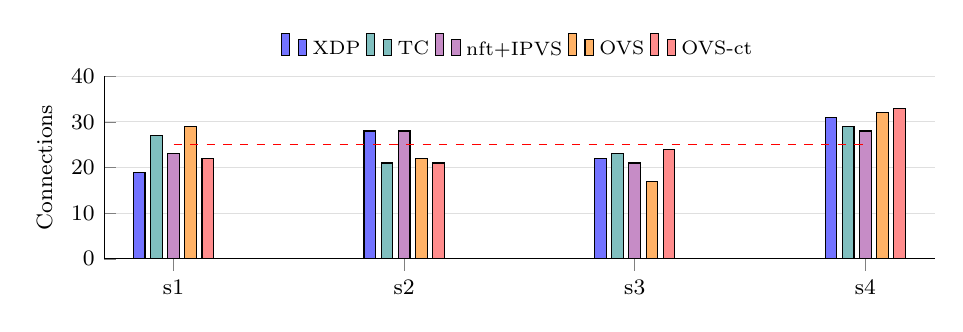
\begin{tikzpicture}
\begin{axis}[ybar, width=\columnwidth, height=3.9cm, bar width=4.2pt,
  symbolic x coords={s1,s2,s3,s4}, xtick=data, ymin=0, ymax=40,
  ylabel={Connections}, axis lines*=left, ymajorgrids, grid style={gray!25},
  legend style={font=\scriptsize, at={(0.5,1.03)}, anchor=south, legend columns=5, draw=none},
  tick label style={font=\footnotesize}, label style={font=\footnotesize}]
\addplot[fill=blue!55] coordinates {(s1,19) (s2,28) (s3,22) (s4,31)};
\addplot[fill=teal!50] coordinates {(s1,27) (s2,21) (s3,23) (s4,29)};
\addplot[fill=violet!45] coordinates {(s1,23) (s2,28) (s3,21) (s4,28)};
\addplot[fill=orange!60] coordinates {(s1,29) (s2,22) (s3,17) (s4,32)};
\addplot[fill=red!45] coordinates {(s1,22) (s2,21) (s3,24) (s4,33)};
\draw[dashed, red] (axis cs:s1,25) -- (axis cs:s4,25);
\legend{XDP, TC, nft+IPVS, OVS, OVS-ct}
\end{axis}
\end{tikzpicture}
\caption{Distribution of 100 new connections to the VIP over four backends
(dashed: ideal 25 per backend).}
\label{fig:dist}
\end{figure}

\subsection{Throughput and Packet Rate}
Table~\ref{tab:perf} lists all measurements and Fig.~\ref{fig:tput} plots
throughput and packet rate. With 10 interleaved rounds, the coefficient of
variation of TCP throughput is 2--10\% per configuration, small enough to
separate the main groups:
\begin{itemize}
\item \textbf{Stateless forwarding} is fastest. Kernel routing reaches
13.72~Gbit/s and 712~kpps; stateless OVS is statistically indistinguishable
from it (TCP $+0.8\%$, $p=0.79$; packet rate $-6.3\%$, $p=0.25$).
\item \textbf{Stateful processing} costs 12.7--31.3\% in every configuration
that tracks connections. Relative to kernel routing, OVS-ct loses 19.5\% of TCP
throughput and 12.7\% of the packet rate, nft+IPVS 27.9\% and 19.0\%, and the
eBPF data plane 28.1--31.3\% and 21.5--29.0\% (all $p<0.002$).
\item \textbf{Among the stateful configurations}, the eBPF data plane at the
TC hook is statistically indistinguishable from the kernel's native
nft+IPVS stack (TC: TCP $-2.4\%$, $p=0.48$, packet rate $-7.5\%$, $p=0.19$;
TC+FIB: $-0.3\%$, $p=0.92$, and $-3.1\%$, $p=0.49$). At the XDP hook its TCP
throughput is also indistinguishable ($-4.7\%$, $p=0.10$), but its packet
rate is 12.4\% lower ($p<0.001$). All eBPF configurations are below OVS-ct:
10.7--14.6\% in TCP throughput and 10.1--18.7\% in packet rate
($p\le0.023$).
\item \textbf{XDP versus TC} shows no significant throughput difference (TCP
$p=0.53$, packet rate $p=0.38$), and in-program FIB forwarding gives no
significant gain over TC alone (TCP $+2.2\%$, $p=0.58$; packet rate $+4.8\%$,
$p=0.50$).
\end{itemize}
The last point corrects our earlier single-run measurement, which suggested a
21.9\% TCP gain from FIB forwarding; with repeated, pinned runs the difference
is within noise. Pinning and the fixed governor also raised all absolute
numbers roughly three-fold compared with unpinned runs, in which the
scheduler placed traffic tools on efficiency cores at reduced frequency.

\begin{table}[t]
\caption{Benchmark results: mean $\pm$ 95\% CI over 10 interleaved rounds
(path $c_1 \to$ gateway $\to s_2$)}
\label{tab:perf}
\centering\scriptsize
\setlength{\tabcolsep}{2.2pt}
\begin{tabular}{@{}lrrrrrr@{}}
\toprule
Config & TCP & 64-B rate & RTT avg & RTT max & VIP conn. & Flood drops$^{*}$ \\
 & (Gbit/s) & (kpps) & ($\mu$s) & ($\mu$s) & (1/s) & (kpps) \\
\midrule
XDP     & 9.43$\pm$0.46 & 506$\pm$21 & 3.8$\pm$1.8 & 34$\pm$9  & 1336$\pm$84  & 880$\pm$32 \\
TC      & 9.65$\pm$0.64 & 534$\pm$66 & 3.4$\pm$1.6 & 32$\pm$9  & 1237$\pm$183 & 953$\pm$31 \\
TC+FIB  & 9.86$\pm$0.53 & 559$\pm$52 & 3.0$\pm$1.4 & 31$\pm$6  & 1272$\pm$158 & 892$\pm$49 \\
Kernel  & 13.72$\pm$0.94 & 712$\pm$45 & 1.9$\pm$0.2 & 25$\pm$5 & --           & -- \\
nft+IPVS & 9.89$\pm$0.39 & 577$\pm$24 & 2.5$\pm$0.7 & 30$\pm$6 & 1322$\pm$87  & 723$\pm$31 \\
OVS     & 13.84$\pm$0.16 & 667$\pm$72 & 2.3$\pm$0.5 & 209$\pm$66 & 1327$\pm$72 & 874$\pm$27 \\
OVS-ct  & 11.04$\pm$0.24 & 622$\pm$11 & 3.5$\pm$1.1 & 218$\pm$112 & 1279$\pm$90 & 899$\pm$19 \\
\bottomrule
\multicolumn{7}{@{}l}{\scriptsize $^{*}$Sender-limited: all flood packets were dropped; see
Section~\ref{sec:kernel-cost}.}
\end{tabular}
\end{table}

\begin{figure}[t]
\centering
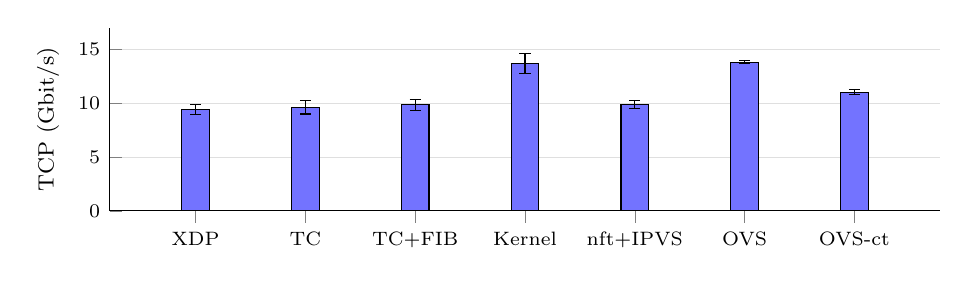
\begin{tikzpicture}
\begin{axis}[benchbar, ylabel={TCP (Gbit/s)}, ymax=17, nodes near coords={},
  error bars/y dir=both, error bars/y explicit]
\addplot[fill=blue!55, error bars/.cd, y dir=both, y explicit] coordinates {
  (XDP,9.43) +- (0,0.46) (TC,9.65) +- (0,0.64) (TC+FIB,9.86) +- (0,0.53)
  (Kernel,13.72) +- (0,0.94) (nft+IPVS,9.89) +- (0,0.39) (OVS,13.84) +- (0,0.16)
  (OVS-ct,11.04) +- (0,0.24)};
\end{axis}
\end{tikzpicture}\\[1mm]
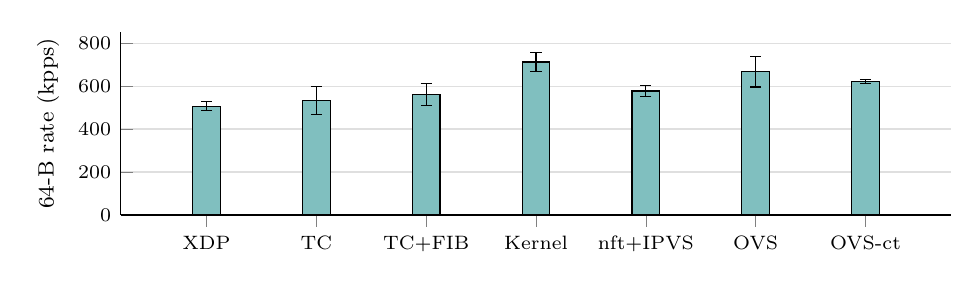
\begin{tikzpicture}
\begin{axis}[benchbar, ylabel={64-B rate (kpps)}, ymax=850, nodes near coords={}]
\addplot[fill=teal!50, error bars/.cd, y dir=both, y explicit] coordinates {
  (XDP,505.7) +- (0,21.3) (TC,533.7) +- (0,65.5) (TC+FIB,559.3) +- (0,51.7)
  (Kernel,712.3) +- (0,45.1) (nft+IPVS,577.2) +- (0,24.3) (OVS,667.3) +- (0,71.5)
  (OVS-ct,621.9) +- (0,10.7)};
\end{axis}
\end{tikzpicture}
\caption{TCP throughput (top) and received 64-byte packet rate (bottom); error
bars are 95\% confidence intervals over 10 rounds.}
\label{fig:tput}
\end{figure}

\subsection{Latency and Connection Rate}
Average round-trip times are 1.9--3.8~$\mu$s in all configurations. They are
close to the 1~$\mu$s resolution of \texttt{ping}, and their confidence
intervals overlap except for kernel routing, which is fastest. Maximum RTTs
separate the designs: both OVS configurations reach 209--218~$\mu$s, versus
25--34~$\mu$s for all others, because the first packet of a flow misses the
OVS kernel cache and is handled by \texttt{ovs-vswitchd} in user space. The
new-connection rate through the VIP is 1237--1336 connections/s for all
load-balancing configurations, with no significant pairwise differences
(e.g., XDP vs.\ nft+IPVS $p=0.79$, XDP vs.\ OVS-ct $p=0.30$); at this level it
is bounded by the user-space HTTP client and server, not by the gateway.

\subsection{In-Kernel Cost and Scalability}
\label{sec:kernel-cost}
Fig.~\ref{fig:scale} shows the per-packet cost of an admitted packet measured
in the kernel. The full pipeline costs 208--259~ns at both hooks, i.e., about
4--5~Mpps per core. With 10\,000 installed rules, which forces all eight IPv4
rule lookups and both L2 lookups to miss, the cost is 214~ns at XDP versus
215~ns with no rules, and 234~ns versus 221~ns at TC; with 60\,000 tracked
connections it is 222~ns versus 212~ns (XDP) and 225~ns versus 224~ns (TC).
Intermediate points vary non-monotonically by up to 17\% (e.g., 259~ns for
100 rules at TC), but the cost does not grow with table size, confirming the
$O(1)$ claim of Section~\ref{sec:complexity} over four orders of magnitude.

Table~\ref{tab:paths} lists the cost of each path. Dropping a packet costs
145--151~ns in the repeat loop, i.e., 6.6--6.9~Mpps per core of in-kernel
drop capacity, far above the 0.7--1.0~Mpps that the Python flood generator
could produce. Load balancing adds 61--71~ns for DNAT and 53--66~ns for SNAT
over the pass path (single-shot measurements, which include about 110~ns of timing
overhead, as the pass path shows: 324~ns single-shot versus 215~ns in the
repeat loop at XDP). The two hooks differ by less than 5\% on every path.

\begin{figure}[t]
\centering
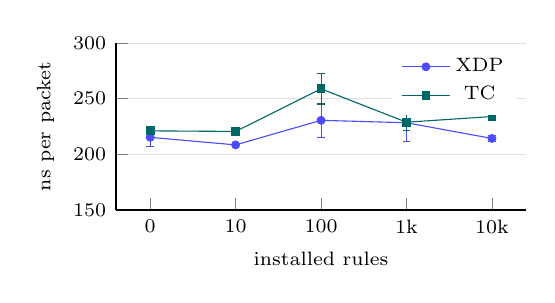
\begin{tikzpicture}
\begin{axis}[width=0.56\columnwidth, height=3.7cm, ymin=150, ymax=300,
  symbolic x coords={0,10,100,1k,10k}, xtick=data, ylabel={ns per packet},
  xlabel={installed rules}, axis lines*=left, ymajorgrids, grid style={gray!25},
  tick label style={font=\scriptsize}, label style={font=\scriptsize},
  legend style={font=\scriptsize, at={(0.98,0.98)}, anchor=north east, draw=none}]
\addplot[blue!70, mark=*, mark size=1.4pt, error bars/.cd, y dir=both, y explicit]
  coordinates {(0,215.3) +- (0,8.0) (10,208.5) +- (0,1.7) (100,230.6) +- (0,15.2)
               (1k,228.4) +- (0,16.8) (10k,214.3) +- (0,2.4)};
\addplot[teal!80!black, mark=square*, mark size=1.4pt, error bars/.cd, y dir=both, y explicit]
  coordinates {(0,221.1) +- (0,3.1) (10,220.6) +- (0,1.5) (100,258.9) +- (0,13.6)
               (1k,228.9) +- (0,7.3) (10k,234.0) +- (0,3.2)};
\legend{XDP, TC}
\end{axis}
\end{tikzpicture}%
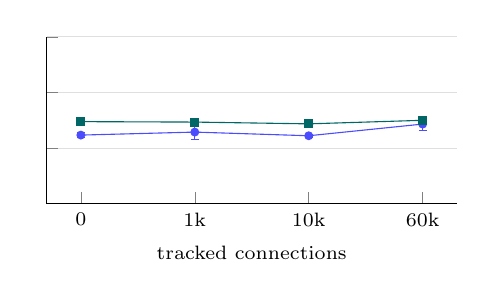
\begin{tikzpicture}
\begin{axis}[width=0.56\columnwidth, height=3.7cm, ymin=150, ymax=300,
  symbolic x coords={0,1k,10k,60k}, xtick=data, yticklabels={},
  xlabel={tracked connections}, axis lines*=left, ymajorgrids, grid style={gray!25},
  tick label style={font=\scriptsize}, label style={font=\scriptsize}]
\addplot[blue!70, mark=*, mark size=1.4pt, error bars/.cd, y dir=both, y explicit]
  coordinates {(0,211.7) +- (0,2.0) (1k,214.4) +- (0,6.7) (10k,211.1) +- (0,1.5)
               (60k,221.6) +- (0,6.1)};
\addplot[teal!80!black, mark=square*, mark size=1.4pt, error bars/.cd, y dir=both, y explicit]
  coordinates {(0,223.8) +- (0,3.0) (1k,223.4) +- (0,3.0) (10k,221.8) +- (0,2.0)
               (60k,225.0) +- (0,2.2)};
\end{axis}
\end{tikzpicture}
\caption{In-kernel cost of an admitted packet versus installed rules (left)
and tracked connections per table (right); mean $\pm$ 95\% CI of 15 samples of
$2\times10^5$ runs each (\texttt{BPF\_PROG\_TEST\_RUN}, performance core,
fixed governor).}
\label{fig:scale}
\end{figure}

\begin{table}[t]
\caption{In-kernel cost per processing path (ns, mean $\pm$ 95\% CI)}
\label{tab:paths}
\centering\scriptsize
\begin{tabular}{@{}lrrrrr@{}}
\toprule
Hook & Pass$^{\dagger}$ & Drop$^{\dagger}$ & Pass & DNAT & SNAT \\
\midrule
XDP & 215.3$\pm$8.0 & 145.1$\pm$1.8 & 324.4$\pm$8.6 & 395.2$\pm$4.0 & 390.0$\pm$5.5 \\
TC  & 221.1$\pm$3.1 & 150.6$\pm$1.0 & 340.4$\pm$7.4 & 401.0$\pm$4.8 & 393.1$\pm$4.7 \\
\bottomrule
\multicolumn{6}{@{}l}{\scriptsize $^{\dagger}$Repeat loop. Other columns: single-shot runs,
including timing overhead.}
\end{tabular}
\end{table}

\textit{Flood test.} Every flood packet was dropped in every configuration, so
the flood rates in Table~\ref{tab:perf} are bounded by the single-threaded
sender. On veth links the gateway's processing runs in the sender's softirq
context on the same core, so the rate still reflects the cost of the drop
path: nft+IPVS, which drops in the forward hook after the routing decision and
the conntrack lookup, sustains 17--24\% lower rates than the eBPF and OVS data
planes, which drop at ingress ($p<0.001$). At XDP, dropping is 7.6\% slower
than at TC ($p=0.002$) because native veth XDP first converts the socket
buffer into an XDP buffer.

\subsection{Discussion}
\textit{Functionality.} With connection tracking, all three stateful designs
provide the required functions: stateful filtering, VIP load balancing with
NAT, graceful draining and in-kernel drop counters. The eBPF design differs in
\emph{how}: one verified program and one set of maps implement the whole
policy, its behaviour is specified by Eqs.~(\ref{eq:patterns})--(\ref{eq:expiry}),
it exports per-flow counters of admitted traffic, and it judges load-balanced
replies by the client-visible flow. The earlier claim that only the eBPF data
plane supports connection tracking and draining held for stateless
OpenFlow~1.3, not for OVS with its conntrack extensions.

\textit{Performance.} On veth links the eBPF data plane performs on par with
the kernel's own stateful stack at the TC hook and 5--12\% below it at XDP,
and 10--19\% below OVS-ct. Two effects explain this. First, XDP's advantage
comes from running in the NIC driver before a socket buffer is allocated; a
veth packet already has one, so native veth XDP must convert it and gains
nothing from early execution. Second, every packet traverses the full
pipeline---about ten rule lookups, connection-table and telemetry updates
(Section~\ref{sec:kernel-cost})---whereas OVS resolves most packets with a
single lookup in its megaflow cache, which already embeds the conntrack state.
A per-flow verdict cache in the eBPF program is the corresponding
optimization.

\subsection{Threats to Validity}
\label{sec:threats}
All links are veth pairs inside one machine, which does not exercise XDP's
driver-level fast path, and the traffic generators share the CPU with the
gateway; pinning and interleaving reduce but do not remove this interference.
Ten rounds bound the uncertainty of each mean (Table~\ref{tab:perf}); smaller
differences, such as among the three eBPF configurations, remain within it.
Disabling checksum offload lowers absolute TCP throughput equally for all
configurations. The HTTP connection rate is bounded by Python servers, and the
flood rate by a Python sender. The microbenchmark measures the program alone,
without driver and stack costs.

%=====================================================================
\section{Conclusion}
%=====================================================================
We designed, implemented and evaluated an eBPF/XDP gateway data plane that
moves the SDN switch into the Linux kernel. One verified pipeline provides a
stateful firewall over the client-visible flow, an L4 load balancer with
DNAT/SNAT, graceful draining and $O(1)$ checksum maintenance, and per-flow
telemetry at either the XDP or the TC hook, and a libbpf-based control plane
reprograms it at runtime and expires connection state like OpenFlow timeouts.
The implementation passes 92 of 93 automated tests (one skipped because of a
kernel test-harness limitation) and every end-to-end scenario at both hooks.
In 10 interleaved, pinned rounds on emulated veth links, it reaches
9.4--9.9~Gbit/s of TCP throughput (28--31\% below plain kernel routing) and
506--559~kpps for 64-byte packets (22--29\% below plain kernel routing),
which at the TC hook is statistically indistinguishable from the kernel's
native nftables and IPVS stack and 10--19\% below OVS with connection
tracking. Measured in the kernel, an admitted packet costs about 0.21--0.23~$\mu$s
and a dropped packet 0.15~$\mu$s, independent of the number of rules
(0--10\,000) and tracked connections (0--60\,000).
Future work will evaluate the system on physical NICs with native XDP support
and hardware traffic generators, add a per-flow verdict cache, replace modulo
hashing with Maglev-style consistent hashing \cite{eisenbud2016maglev} to
reduce remapping when pools change, and add prefix (LPM) rules.

%=====================================================================
\begin{thebibliography}{00}
\bibitem{kreutz2015sdn} D. Kreutz, F. M. V. Ramos, P. E. Ver\'issimo,
C. E. Rothenberg, S. Azodolmolky, and S. Uhlig, ``Software-defined networking:
A comprehensive survey,'' \textit{Proc. IEEE}, vol.~103, no.~1, pp.~14--76,
Jan. 2015, doi: 10.1109/JPROC.2014.2371999.

\bibitem{feamster2014road} N. Feamster, J. Rexford, and E. Zegura, ``The road
to SDN: An intellectual history of programmable networks,'' \textit{ACM
SIGCOMM Comput. Commun. Rev.}, vol.~44, no.~2, pp.~87--98, Apr. 2014.

\bibitem{mckeown2008openflow} N. McKeown, T. Anderson, H. Balakrishnan,
G. Parulkar, L. Peterson, J. Rexford, S. Shenker, and J. Turner, ``OpenFlow:
Enabling innovation in campus networks,'' \textit{ACM SIGCOMM Comput. Commun.
Rev.}, vol.~38, no.~2, pp.~69--74, Apr. 2008, doi: 10.1145/1355734.1355746.

\bibitem{pfaff2015ovs} B. Pfaff, J. Pettit, T. Koponen, E. Jackson, A. Zhou,
J. Rajahalme, J. Gross, A. Wang, J. Stringer, P. Shelar, K. Amidon, and
M. Casado, ``The design and implementation of Open vSwitch,'' in \textit{Proc.
12th USENIX Symp. Netw. Syst. Design Implement. (NSDI)}, Oakland, CA, USA,
2015, pp.~117--130.

\bibitem{hoiland2018xdp} T. H{\o}iland-J{\o}rgensen, J. D. Brouer,
D. Borkmann, J. Fastabend, T. Herbert, D. Ahern, and D. Miller, ``The eXpress
data path: Fast programmable packet processing in the operating system
kernel,'' in \textit{Proc. 14th Int. Conf. Emerg. Netw. Exp. Technol.
(CoNEXT)}, Heraklion, Greece, 2018, pp.~54--66, doi: 10.1145/3281411.3281443.

\bibitem{vieira2020ebpf} M. A. M. Vieira, M. S. Castanho, R. D. G. Pac\'ifico,
E. R. S. Santos, E. P. M. C\^amara J\'unior, and L. F. M. Vieira, ``Fast packet
processing with eBPF and XDP: Concepts, code, challenges, and applications,''
\textit{ACM Comput. Surv.}, vol.~53, no.~1, pp.~1--36, Feb. 2020,
doi: 10.1145/3371038.

\bibitem{cilium} Cilium Authors, ``Cilium: eBPF-based networking,
observability, and security,'' 2025. [Online]. Available:
https://cilium.io (accessed Nov. 17, 2026).

\bibitem{katran} Meta Platforms, ``Katran: A high performance layer 4 load
balancer,'' 2025. [Online]. Available:
https://github.com/facebookincubator/katran (accessed Nov. 17, 2026).

\bibitem{miano2021polycube} S. Miano, F. Risso, M. V. Bernal, M. Bertrone, and
Y. Lu, ``A framework for eBPF-based network functions in an era of
microservices,'' \textit{IEEE Trans. Netw. Service Manag.}, vol.~18, no.~1,
pp.~133--151, Mar. 2021, doi: 10.1109/TNSM.2021.3055676.

\bibitem{bosshart2014p4} P. Bosshart, D. Daly, G. Gibb, M. Izzard,
N. McKeown, J. Rexford, C. Schlesinger, D. Talayco, A. Vahdat, G. Varghese,
and D. Walker, ``P4: Programming protocol-independent packet processors,''
\textit{ACM SIGCOMM Comput. Commun. Rev.}, vol.~44, no.~3, pp.~87--95,
Jul. 2014, doi: 10.1145/2656877.2656890.

\bibitem{tu2021ovs} W. Tu, Y.-H. Wei, G. Antichi, and B. Pfaff, ``Revisiting
the Open vSwitch dataplane ten years later,'' in \textit{Proc. ACM SIGCOMM
Conf.}, 2021, pp.~245--257, doi: 10.1145/3452296.3472914.

\bibitem{chaignon2018oko} P. Chaignon, K. Lazri, J. Fran\c{c}ois, T. Delmas,
and O. Festor, ``Oko: Extending Open vSwitch with stateful filters,'' in
\textit{Proc. Symp. SDN Res. (SOSR)}, Los Angeles, CA, USA, 2018, pp.~1--13,
doi: 10.1145/3185467.3185496.

\bibitem{miano2018creating} S. Miano, M. Bertrone, F. Risso, M. Tumolo, and
M. V. Bernal, ``Creating complex network services with eBPF: Experience and
lessons learned,'' in \textit{Proc. IEEE 19th Int. Conf. High Perform.
Switching Routing (HPSR)}, Bucharest, Romania, 2018, pp.~1--8.

\bibitem{miano2019bpfiptables} S. Miano, M. Bertrone, F. Risso, M. V. Bernal,
Y. Lu, and J. Pi, ``Securing Linux with a faster and scalable iptables,''
\textit{ACM SIGCOMM Comput. Commun. Rev.}, vol.~49, no.~3, pp.~2--17,
Jul. 2019, doi: 10.1145/3371927.3371929.

\bibitem{scholz2018filtering} D. Scholz, D. Raumer, P. Emmerich, A. Kurtz,
K. Lesiak, and G. Carle, ``Performance implications of packet filtering with
Linux eBPF,'' in \textit{Proc. 30th Int. Teletraffic Congr. (ITC)}, Vienna,
Austria, 2018, pp.~209--217.

\bibitem{nftables} Netfilter Project, ``nftables,'' 2025. [Online].
Available: https://netfilter.org/projects/nftables/ (accessed Nov. 17, 2026).

\bibitem{zhang2000lvs} W. Zhang, ``Linux Virtual Server for scalable network
services,'' in \textit{Proc. Ottawa Linux Symp.}, Ottawa, ON, Canada,
Jul. 2000.

\bibitem{eisenbud2016maglev} D. E. Eisenbud, C. Yi, C. Contavalli, C. Smith,
R. Kononov, E. Mann-Hielscher, A. Cilingiroglu, B. Cheyney, W. Shang, and
J. D. Hosein, ``Maglev: A fast and reliable software network load balancer,''
in \textit{Proc. 13th USENIX Symp. Netw. Syst. Design Implement. (NSDI)},
Santa Clara, CA, USA, 2016, pp.~523--535.

\bibitem{srinivasan1999tss} V. Srinivasan, S. Suri, and G. Varghese, ``Packet
classification using tuple space search,'' in \textit{Proc. ACM SIGCOMM
Conf.}, Cambridge, MA, USA, 1999, pp.~135--146, doi: 10.1145/316188.316216.

\bibitem{lantz2010mininet} B. Lantz, B. Heller, and N. McKeown, ``A network in
a laptop: Rapid prototyping for software-defined networks,'' in \textit{Proc.
9th ACM SIGCOMM Workshop Hot Topics Netw. (HotNets)}, Monterey, CA, USA, 2010,
Art. no.~19, doi: 10.1145/1868447.1868466.

\bibitem{rfc1624} A. Rijsinghani, ``Computation of the Internet checksum via
incremental update,'' RFC 1624, IETF, May 1994.

\bibitem{rfc1071} R. Braden, D. Borman, and C. Partridge, ``Computing the
Internet checksum,'' RFC 1071, IETF, Sep. 1988.

\bibitem{rfc768} J. Postel, ``User datagram protocol,'' RFC 768, IETF,
Aug. 1980.
\end{thebibliography}

\end{document}
